\documentclass[11pt]{article}

\newcommand{\HWnum}{3} 
\newcommand{\StudName}{Timothy Holmes} % author
\newcommand{\CourseNum}{411}           % course number
\newcommand{\Subject}{PHY}

\usepackage{graphicx, amsmath, amssymb,fancyhdr}
\addtolength{\textwidth}{1.5in}
\addtolength{\oddsidemargin}{-2cm}
\addtolength{\evensidemargin}{-2cm}
\addtolength{\textheight}{1.6in}
\addtolength{\topmargin}{-0.7in}
\addtolength{\headsep}{-0.1in}
%\addtolength{\footskip}{-0.2in}
\pagestyle{fancy}
\cfoot{}
\lhead{\textbf{\Subject~\CourseNum~--- Homework~\HWnum}}
\rhead{\textbf{\StudName:~Page~\thepage}}

\addtolength{\parskip}{\baselineskip} % skips a line between paragraphs
\parindent 0in                        % no indent at start of paragraph

\newcommand{\dd}{\textrm{d}}
\usepackage{braket}
\usepackage{lipsum, babel}
\usepackage{blindtext}
\usepackage{graphicx}% Include figure files
\usepackage{dcolumn}% Align table columns on decimal point
\usepackage{bm}% bold math
\usepackage{listings}
\usepackage{listing}
\usepackage{supertabular}



\usepackage{color} %red, green, blue, yellow, cyan, magenta, black, white
\definecolor{mygreen}{RGB}{28,172,0} % color values Red, Green, Blue
\definecolor{mylilas}{RGB}{170,55,241}



\lstset{language=Python,%
    %basicstyle=\color{red},
    breaklines=true,%
    morekeywords={matlab2tikz},
    keywordstyle=\color{blue},%
    morekeywords=[2]{1}, keywordstyle=[2]{\color{black}},
    identifierstyle=\color{black},%
    stringstyle=\color{mylilas},
    commentstyle=\color{mygreen},%
    showstringspaces=false,%without this there will be a symbol in the places where there is a space
    numbers=left,%
    numberstyle={\tiny \color{black}},% size of the numbers
    numbersep=9pt, % this defines how far the numbers are from the text
    emph=[1]{for,end,break},emphstyle=[1]\color{red}, %some words to emphasise
    %emph=[2]{word1,word2}, emphstyle=[2]{style},    
}


\begin{document}
% -------------------------- BOD -------------------------- 

\title{Homework {\HWnum}}
\author{Timothy Holmes \\ \Subject~411 Electrodynamics I}

\maketitle

\section*{Problem 1}

Show 

$$
\Bigg[\frac{1}{\mu}(\vec{k} \times \vec{E_{0}} + \vec{k}'' \times \vec{E_{0}}'') - \frac{1}{\mu'}(\vec{k}' \times \vec{E_{0}'})\Bigg] \times \hat{n} = 0
$$

Reduces to 

$$
\Bigg[\sqrt{\frac{\epsilon}{\mu}}E_{0}cos(i) - \sqrt{\frac{\epsilon}{\mu}}E_{0}''cos(i) - 
\sqrt{\frac{\epsilon'}{\mu'}}E_{0}'cos(r)\Bigg] = 0.
$$

Starting from the first equation, it can be expanded to 

$$
\Bigg[\frac{1}{\mu}(\vec{k} \times \vec{E_{0}}) + \frac{1}{\mu}(\vec{k}'' \times \vec{E_{0}}'') - \frac{1}{\mu'}(\vec{k}' \times \vec{E_{0}'})\Bigg] \times \hat{n} = 0.
$$

the energy flow is in the direction of the \vec{k}, so the curl from $\vec{E}$ is $\vec{B}$. Therefore, $\vec{k} \times \vec{E_{0}}$ will become $\vec{B}$, $\vec{k}'' \times \vec{E_{0}}''$ will become $\vec{B}''$, and $\vec{k}' \times \vec{E_{0}}'$ will become $\vec{B}'$. Therefore, the equation becomes

$$
\Bigg[\frac{1}{\mu}(\vec{B_{0}} \times \hat{n}) + \frac{1}{\mu}(\vec{B_{0}}'' \times \hat{n}) - \frac{1}{\mu'}(\vec{B_{0}}' \times \hat{n})\Bigg] = 0.
$$

$\vec{B_{0}}$ is now perpendicular to the field so this means that all the $B_{0}$ vectors are $B_{0}cos(i)$. Therefore, we have, for one example of $\vec{B_{0}}$ that

$$
\frac{1}{\mu}(\vec{B_{0}} \times \hat{n}) = \frac{1}{\mu}\vec{B_{0}}cos(i)
$$

which can also be expressed as

$$
\frac{1}{\mu}(\vec{B_{0}} \times \hat{n}) = \frac{\sqrt{\mu\epsilon}}{\mu}\vec{E_{0}}cos(i)
$$

and reduced to

$$
\frac{1}{\mu}(\vec{B_{0}} \times \hat{n}) = \sqrt{\frac{\epsilon}{\mu}}\vec{E_{0}}cos(i).
$$

Thus, the final equation is then 

$$
\Bigg[\sqrt{\frac{\epsilon}{\mu}}E_{0}cos(i) - \sqrt{\frac{\epsilon}{\mu}}E_{0}''cos(i) - 
\sqrt{\frac{\epsilon'}{\mu'}}E_{0}'cos(r)\Bigg] = 0.
$$

% If you insert the command below
\clearpage

\section*{Problem 2}

Since 

$$
E_{0} + E''_{0} - E'_{0} = 0
$$

and 

$$
\Bigg[\sqrt{\frac{\epsilon}{\mu}}E_{0}cos(i) - \sqrt{\frac{\epsilon}{\mu}}E_{0}''cos(i) - 
\sqrt{\frac{\epsilon'}{\mu'}}E_{0}'cos(r)\Bigg] = 0.
$$

The equation above can be reduced to 

$$
\sqrt{\frac{\epsilon}{\mu}}(E_{0} - E_{0}'')cos(i) - 
\sqrt{\frac{\epsilon'}{\mu'}}E_{0}'cos(r) = 0.
$$

Now, $E_{0} + E''_{0} - E'_{0} = 0$ can also be rewrote as $E_{0} + E''_{0} = E'_{0}$ and the equation will become

$$
\sqrt{\frac{\epsilon}{\mu}}(E_{0} - E_{0}'')cos(i) = 
\sqrt{\frac{\epsilon'}{\mu'}}(E_{0} - E''_{0})cos(r).
$$

From equation 7.36 we know that 

$$
\frac{sin(i)}{sin(r)} = \frac{k'}{k} = \sqrt{\frac{\mu'\epsilon'}{\mu\epsilon}} = \frac{n'}{n}.
$$

From equation 7.44 it can be worked out that

$$
i_{0} = sin^{-1}\Bigg(\frac{n'}{n}\Bigg) \rightarrow sin(i_{0}) = \Bigg(\frac{n'}{n}\Bigg) \rightarrow sin(i_{0}) = \Bigg(\frac{sin(i)}{sin(r)}\Bigg) \rightarrow sin(r) = \Bigg(\frac{sin(i)}{sin(i_{0})}\Bigg)
$$
Finally, equation 7.45 says that 

$$
cos(r) = i\sqrt{\Bigg(\frac{sin(i)}{sin(i_{0}}\Bigg) - 1} 
$$

$$
cos(r) = \sqrt{1 - \Bigg(\frac{sin(i)}{sin(i_{0}}\Bigg)} 
$$

$$
cos(r) = \sqrt{1 - \frac{n^{2}}{n'^{2}}sin^{2}(i)} 
$$

$$
cos(r) = \frac{\sqrt{n'^{2} - n^{2}sin^{2}(i)}}{n}.
$$

Therefore, the equation becomes

$$
\sqrt{\frac{\epsilon}{\mu}}(E_{0} - E_{0}'')cos(i) = \sqrt{\frac{\epsilon'}{\mu'}}(E_{0} - E''_{0})\frac{\sqrt{n'^{2} - n^{2}sin^{2}(i)}}{n}.
$$

Expanding the equation result in 

$$
\sqrt{\frac{\epsilon}{\mu}}E_{0}cos(i) - \sqrt{\frac{\epsilon}{\mu}}E_{0}''cos(i) = \sqrt{\frac{\epsilon'}{\mu'}}E_{0}\frac{\sqrt{n'^{2} - n^{2}sin^{2}(i)}}{n} + \sqrt{\frac{\epsilon'}{\mu'}}E''_{0}\frac{\sqrt{n'^{2} - n^{2}sin^{2}(i)}}{n}.
$$

The idea here is to combine the $E$ terms to be on one specific side such that the equation becomes

$$
\sqrt{\frac{\epsilon}{\mu}}E_{0}cos(i) - \sqrt{\frac{\epsilon'}{\mu'}}E_{0}\frac{\sqrt{n'^{2} - n^{2}sin^{2}(i)}}{n} = \sqrt{\frac{\epsilon}{\mu}}E_{0}''cos(i) + \sqrt{\frac{\epsilon'}{\mu'}}E''_{0}\frac{\sqrt{n'^{2} - n^{2}sin^{2}(i)}}{n}
$$

and then is factored so that 

$$
E_{0}\Bigg(\sqrt{\frac{\epsilon}{\mu}}cos(i) - \sqrt{\frac{\epsilon'}{\mu'}}\frac{\sqrt{n'^{2} - n^{2}sin^{2}(i)}}{n}\Bigg)= E''_{0}\Bigg(\sqrt{\frac{\epsilon}{\mu}}cos(i) + \sqrt{\frac{\epsilon'}{\mu'}}\frac{\sqrt{n'^{2} - n^{2}sin^{2}(i)}}{n}\Bigg).
$$

Remembering that $\sqrt{\mu'\epsilon'/ \mu\epsilon}$, we arrive at the equation

$$
\frac{E''_{0}}{E_{0}} = \frac{ncos(i) - (\mu/\mu')\sqrt{n'^{2} - n^{2}sin^{2}(i)}}{ncos(i) - (\mu/\mu')\sqrt{n'^{2} - n^{2}sin^{2}(i)}}.
$$

Similarly, if we let $E''_{0} = (E'_{0} - E_{0})$ then 

$$
\Bigg[\sqrt{\frac{\epsilon}{\mu}}E_{0}cos(i) - \sqrt{\frac{\epsilon}{\mu}}(E'_{0} - E_{0})cos(i) - 
\sqrt{\frac{\epsilon'}{\mu'}}E_{0}'cos(r)\Bigg] = 0.
$$

Expanding and collecting like terms allow us to rewrite the equation as

$$
\sqrt{\frac{\epsilon}{\mu}}(2E_{0} - E'_{0})cos(i) =
\sqrt{\frac{\epsilon'}{\mu'}}E_{0}'cos(r).
$$

Separating the $E$ values to each side gives us

$$
2\sqrt{\frac{\epsilon}{\mu}}E_{0}cos(i) = \sqrt{\frac{\epsilon'}{\mu'}}E_{0}'cos(r) + \sqrt{\frac{\epsilon}{\mu}}E_{0}'cos(i)
$$

$$
2\sqrt{\frac{\epsilon}{\mu}}E_{0}cos(i) = E_{0}\Bigg(\sqrt{\frac{\epsilon'}{\mu'}}cos(r) + \sqrt{\frac{\epsilon}{\mu}}cos(i)\Bigg)
$$

We can rewrite the equation as

$$
\frac{E'_{0}}{E_{0}} = \frac{2\sqrt{\epsilon/\mu} cos(i)}{\sqrt{\epsilon/\mu} cos(i) + \sqrt{\epsilon'/\mu'}cos(r)}
$$

Remember that 

$$
cos(r) = \frac{\sqrt{n'^{2} - n^{2}sin^{2}(i)}}{n}.
$$

and 

$$
\sqrt{\frac{\epsilon'}{\epsilon}} = \frac{n'}{n}.
$$

Thus, the final equation will becomes

$$
\frac{E'_{0}}{E_{0}} = \frac{2nn'cos(i)}{ncos(i) - (\mu/\mu')\sqrt{n'^{2} - n^{2}sin^{2}(i)}}.
$$

\clearpage

\section*{Problem 3}

The transmission coefficient is gave by equation 7.13c in the class summaries as

$$
T = \frac{\vec{s}' \cdot \hat{n}}{\vec{s} \cdot \hat{n}}.
$$

The equation $\vec{s}$, $\vec{s}'$, and $\vec{s}''$ and are gave as 

$$
\vec{s} = \frac{1}{2}\sqrt{\frac{\epsilon}{\mu}}|E_{0}|^{2}\hat{k}
$$

$$
\vec{s}' = \frac{1}{2}\sqrt{\frac{\epsilon'}{\mu'}}|E_{0}'|^{2}\hat{k}
$$

$$
\vec{s}'' = \frac{1}{2}\sqrt{\frac{\epsilon}{\mu}}|E_{0}''|^{2}\hat{k}
$$

Now when taking the dot product of the vectors above with the unit vector $\hat{n}$, the following are the results

$$
\vec{s} \cdot \hat{n} = \frac{1}{2}\sqrt{\frac{\epsilon}{\mu}}|E_{0}|^{2}cos(i)
$$

$$
\vec{s}' \cdot \hat{n} = \frac{1}{2}\sqrt{\frac{\epsilon'}{\mu'}}|E_{0}'|^{2}\cos(r)
$$

$$
\vec{s}'' \cdot \hat{n} = \frac{1}{2}\sqrt{\frac{\epsilon}{\mu}}|E_{0}''|^{2}\cos(r)'
$$

Therefore, the transmission coefficient becomes

$$
T = \sqrt{\frac{\epsilon'}{\mu'}} \sqrt{\frac{\epsilon}{\mu}} \frac{1}{2} \frac{2}{1} \frac{|E_{0}'|^{2}}{|E_{0}|^{2}} \frac{cos(r)}{cos(i)}
$$

Remember that $cos(r)$ is

$$
cos(r) = \frac{\sqrt{n'^{2} - n^{2}sin^{2}(i)}}{n}
$$

then $T$ becomes 

$$
T = \frac{|E_{0}'|^{2}}{|E_{0}|^{2}} \frac{\sqrt{n'^{2} - n^{2}sin^{2}(i)}}{ncos(i)}.
$$

Since we are going to assume that $\mu = \mu'$ and $E'_{0}/E_{0}$ from equation 7.41, T is now 

$$
T = \Bigg|\frac{2nn'cos(i)}{n'^{2}cos(i) + n\sqrt(n'^{2}sin^{2}(i)}\Bigg|^{2}\frac{\sqrt{n'^{2} - n^{2}sin^{2}(i)}}{ncos(i)}
$$

Similarly, the reflection coefficient is 
$$
R = \frac{\vec{s}'' \cdot \hat{n}}{\vec{s} \cdot \hat{n}}.
$$

Following the same method $R$ becomes

$$
R = \sqrt{\frac{\mu}{\mu'}} \sqrt{\frac{\epsilon}{\epsilon'}} \frac{1}{2} \frac{2}{1} \frac{|E''_{0}|^{2}}{|E_{0}|^{2}} \frac{cos(r')}{cos(i)}.
$$


Remember that $\mu = \mu'$ and $\epsilon = \epsilon'$, since we are in the same medium, the equation is reduced to

$$
R =\Bigg|\frac{n'^{2}cos(i)-n\sqrt{n'^{2}-n^{2}sin^{2}(i)}}{n'^{2}cos(i)+n\sqrt{n'^{2}-n^{2}sin^{2}(i)}}\Bigg|^{2} \frac{cos(r')}{cos(i)}.
$$

The angle $i$ is equal to $r'$, therefore $cos(r')$ can be wrote as $cos(i)$. The $cos(i)$ will cancel out and the final equation becomes,

$$
R =\Bigg|\frac{n'^{2}cos(i)-n\sqrt{n'^{2}-n^{2}sin^{2}(i)}}{n'^{2}cos(i)+n\sqrt{n'^{2}-n^{2}sin^{2}(i)}}\Bigg|^{2}.
$$

\clearpage

\section*{Problem 4}

\begin{center}
    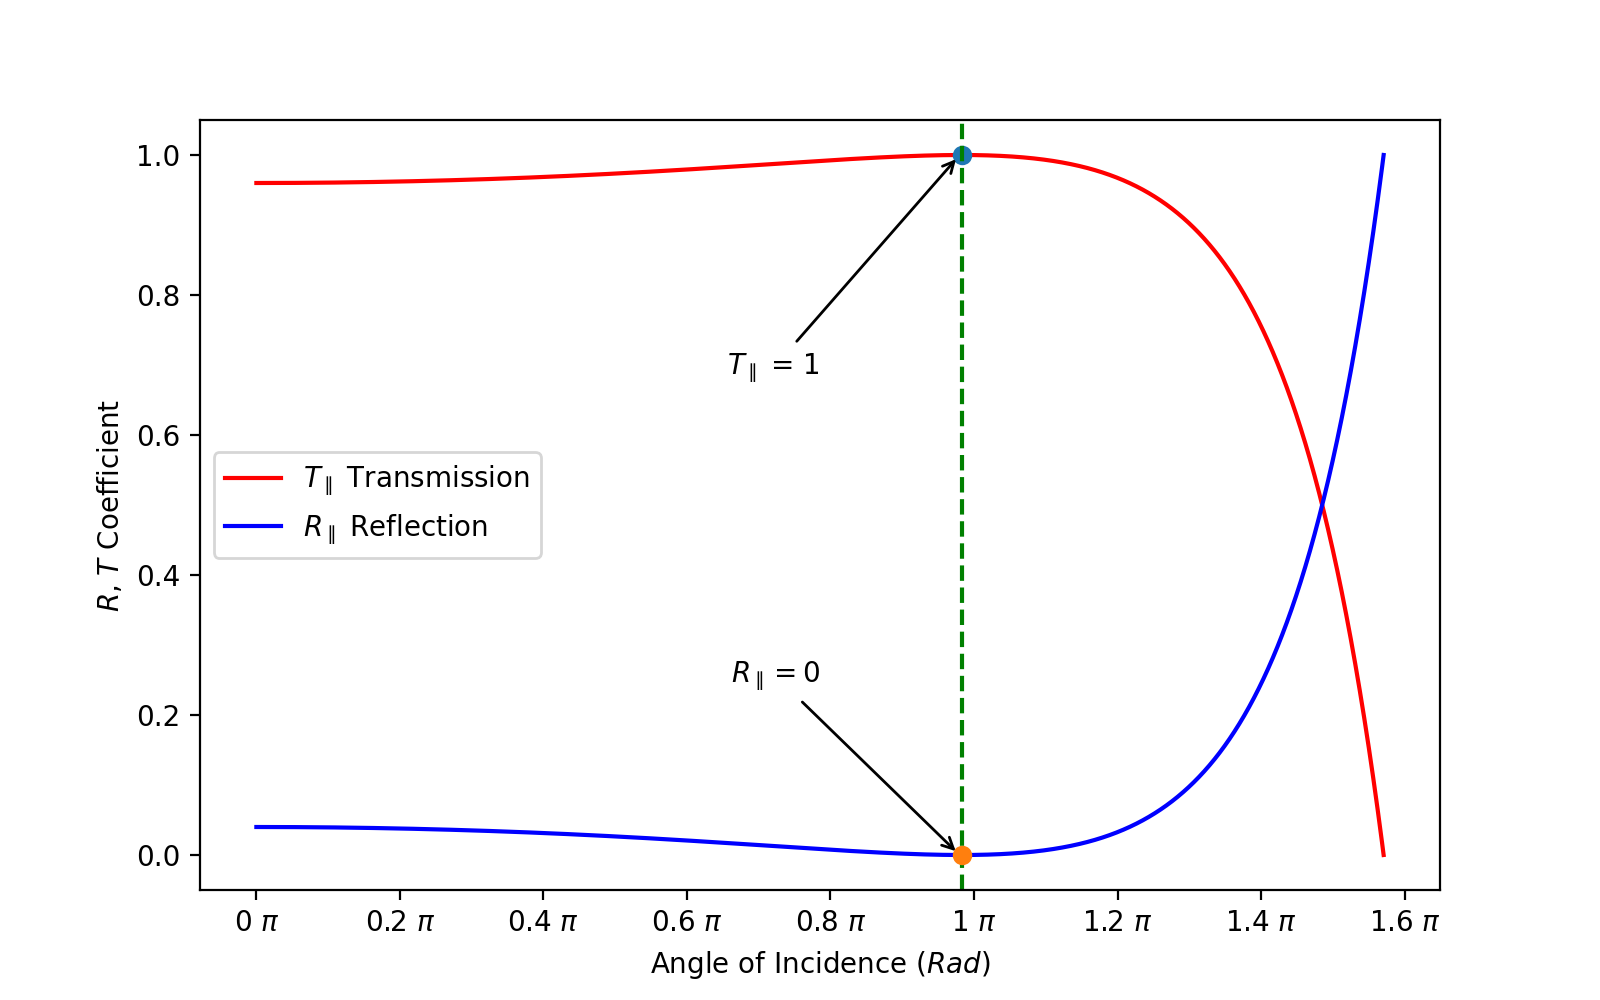
\includegraphics[width=1.0\textwidth]{t_r_plot.png}
    \caption{\small FIG 1: .}
\end{center}

FIG 1. shows the reflective coefficient in blue and the transmission coefficient in red. Starting from the when the angle of incidence is $0^{\circ}$, $T_{\parallel}$ is not $1$ and $R_{\parallel}$ is not $0$. Intuitively, it would be thought that $T_{\parallel} = 1$ and $R_{\parallel} = 0$ when the angle of incidence is $0^{\circ}$. As the angle of incidence increases and reaches $\approx 56^{\circ}$, then $T_{\parallel} = 1$ and $R_{\parallel} = 0$. Increasing the angle further, the blue and red lines intersect which means that $T_{\parallel} = R_{\parallel}$, until the angle gets to $\pi/2$ in this case $T_{\parallel} = 0$ and $R_{\parallel} = 1$. The reason why $T_{\parallel} = 1$ and $R_{\parallel} = 0$ at $\approx 56^{\circ}$ is due to the Brewster angle. The specific conditions that need to be met are; $n = 1$, $n' = 1.5$, and $\mu = \mu'$. Moreover, the Brewster angle is gave by and for this example is 

$$
i_{B} = tan^{-1}\Bigg(\frac{n'}{n}\Bigg) = tan^{-1}\Bigg(\frac{1.5}{1}\Bigg) \approx 56^{\circ}.
$$

At this angle the 100\% of the light is transmitted through the surface while 0\% is reflected.

\clearpage

\section*{Appendix}

\subsection*{Transmission Coefficient and Reflection Coefficient Plot}
\lstinputlisting{homework3.py}

\clearpage
% -------------------------- EOD -------------------------- 
\end{document}